\newpage
\section{Introdução}

\subsection{Conversores \textit{Boost}}
Um conversor do tipo Boost é um conversor DC/DC onde a principal característica é que a tensão de saída é maior que a tensão de entrada. Essa topologia é utilizada por uma grande classe de conversores chaveados e contém no mínimo dois semicondutores (um diodo e um transistor), um elemento de armazenamento de energia (neste caso um indutor) e um filtro (um capacitor para reduzir o ripple na tensão de saída).

A alimentação do conversor Boost poder ser feita através de qualquer fonte DC, tais como baterias, paineis solares, geradores DC ou através da própria rede, depois de retificada e filtrada.
Esse conversor é muitas vezes chamado de \textit{step-up converter}, pois ele eleva (\textit{step-up}) a tensão de entrada. Nestes conversores, para que haja à conservação da energia, a corrente de saída é menor que a corrente de entrada, assim, um ganho em tensão representa uma redução da corrente disponível.

Como o objetivos dos conversores chaveados (\textit{Switched Mode Power Supply}) é a alta eficiência, faz-se necessário o uso de semicondutores de potência de alta frequência. Por isso, tais conversores só se tornaram amplamente utilizados a partir dos anos 50, onde o avanço na industria dos semicondutores tornou prático o emprego do conversor Boost em produtos comerciais, militares e  aeroespaciais. Hoje em dia, os conversores do tipo Boost são amplamente utilizados nos mais diversos aparelhos como celulares, televisores, carros e etc. 

A figura \ref{fig:boost} mostra a topologia básica do conversor \textit{boost}.

\begin{figure}[H]
  \centering
  \caption{Topologia \textit{Boost}.}
  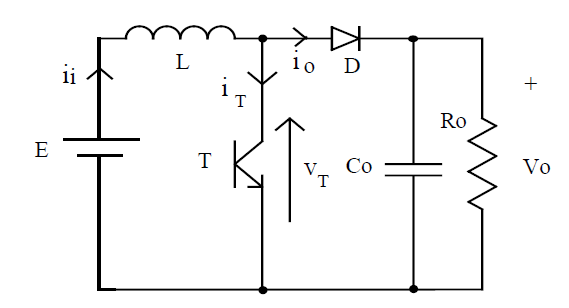
\includegraphics[scale=0.5]{boost}
  \label{fig:boost}
  
  \small Fonte: C. H. G. Treviso, Apostila Eletrônica de Potência \cite{apostila}.
\end{figure}

\subsection{Conversores \textit{Flyback}}
Os conversores do tipo \textit{Flyback} possuem topologia semelhante aos conversores \textit{Buck-Boost}, porém, o mesmo pode ter isolação galvânica, com o uso de um transformador. Sendo assim, é necessário utilizar um elemento que isole a saída de referência do secundário, sendo utilizado, geralmente, um acoplador óptico (fotoacoplador).

Esse conversor é empregado quando há necessidade de elevar ou abaixar a tensão de saída.

A figura \ref{fig:flyback} mostra a topologia básica do conversor \textit{flyback}.

\begin{figure}[H]
  \centering
  \caption{Topologia \textit{Flyback}.}
  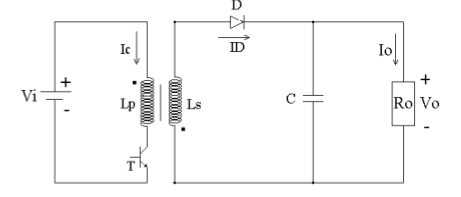
\includegraphics[scale=0.5]{flyback}
  \label{fig:flyback}
  
  \small Fonte: C. H. G. Treviso, Apostila Eletrônica de Potência \cite{apostila}.
\end{figure}

\subsection{Circuito integrado 3525}
O circuito integrado 3525 é um circuito de controle com um modulador PWM que oferece uma boa performance e necessita de poucas partes externas para controlar todos os tipos de fonte chaveada. 

O CI possui uma tensão de referência de +5.1V \textit{on-chip}, i.e., dentro do integrado, a qual possui tolerância de 1\% e elimina a necessidade de um divisor resistivo externo. Outra característica é que o mesmo possibilita o sincronismo entre várias unidades do CI, eliminando ruídos causados pela diferença de clock.

Uma grande variedade de \textit{deadtimes} (tempo morto) podem ser programados utilizando somente um resistor, entre o pino CT e o pino de descarga. 

Para grandes potências, é necessário o uso de um circuito de \textit{softstart}, que no caso ja vem integrado no CI, sendo as funções de \textit{softstart} controladas por um pino de \textit{shutdown}. Esse pino também permite desligar o circuito de PWM instantaneamente, em caso de falha ou outro problema como temperatura muito alta.

A figura mostra o diagrama de blocos do CI SG3525A, fabricado pela ON Semiconductor.

\begin{figure}[H]
  \centering
  \caption{Diagrama de blocos do CI SG3525A.}
  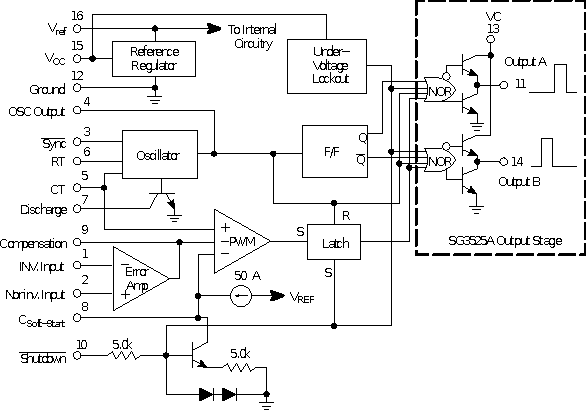
\includegraphics[scale=1]{sg3525a}
  \label{fig:sg3525a}
  
  \small Fonte: Datasheet SG3525A \cite{sg3525a}.
\end{figure}
